\documentclass[10pt,a4paper]{article}
\usepackage{tocloft}
\usepackage{commons/course}  % همین کافیه؛ listings و xcolor داخلشه
\usepackage{booktabs}

% Define colors for syntax highlighting
\definecolor{keywordstyle}{rgb}{0.0, 0.4, 0.8} % A bluer shade
\definecolor{stringstyle}{rgb}{0.9, 0.17, 0.31} % amaranth
\definecolor{commentstyle}{rgb}{0.1, 0.6, 0.2} % green
\definecolor{numberstyle}{rgb}{0.4, 0.4, 0.4} % gray
\definecolor{backgroundcolor}{rgb}{0.94, 0.97, 1.0} % aliceblue

% Define the Python-like language for syntax highlighting
\lstdefinelanguage{PythonLike}{
	morekeywords={mov, add, sub, cmp, jmp , lw , addi,sw,bne},
	sensitive=false,
	morecomment=[l]{;},
	morestring=[b]",
}

% Set the style for Python-like code
\lstset{
	language=PythonLike,
	basicstyle=\ttfamily\small,
	keywordstyle=\color{keywordstyle},
	stringstyle=\color{stringstyle},
	commentstyle=\color{commentstyle},
	numbers=left,
	numberstyle=\tiny\color{numberstyle},
	stepnumber=1,
	numbersep=5pt,
	keepspaces=true,
	tabsize=4,
	showspaces=false,
	showstringspaces=false,
	showtabs=false,
	breaklines=true,
	breakatwhitespace=false,
	frame=single,
	backgroundcolor=\color{backgroundcolor},
}

\newlistof{listofproblems}{lop}{\normalsize فهرست مسائل}
\newcommand{\addproblem}[1]{\addcontentsline{lop}{listofproblems}{\protect\numberline{}#1}}


\begin{document}


\سربرگ{آزمایش اول}{جمع‌کننده دهدهی}{معین آعلی - ثمین اکبری}{استاد: دکتر حمید سربازی آزاد}

\subsubsection*{خلاصه}

در این آزمایش یک جمع‌کننده‌ی دهدهی سه‌رقمی (\lr{3-digit BCD Adder}) در نرم‌افزار \lr{Logisim} طراحی و پیاده‌سازی شده است. مدار به‌صورت سلسله‌مراتبی و از پایین به بالا ساخته شده: یک تمام‌جمع‌کننده‌ی ۱ بیتی (\lr{full\_adder})، که پایه‌ی ساخت یک جمع‌کننده‌ی یک‌رقمی دهدهی با تصحیح خودکار \lr{BCD} (\lr{bcd\_digit}) است، و در نهایت سه نمونه از این جمع‌کننده‌ی رقمی برای ساخت یک جمع‌کننده‌ی سه‌رقمی کامل زنجیر شده‌اند.



\subsubsection*{ دیاگرام یک جمع‌کننده دهدهی}
\begin{figure}[h]
  \centering
  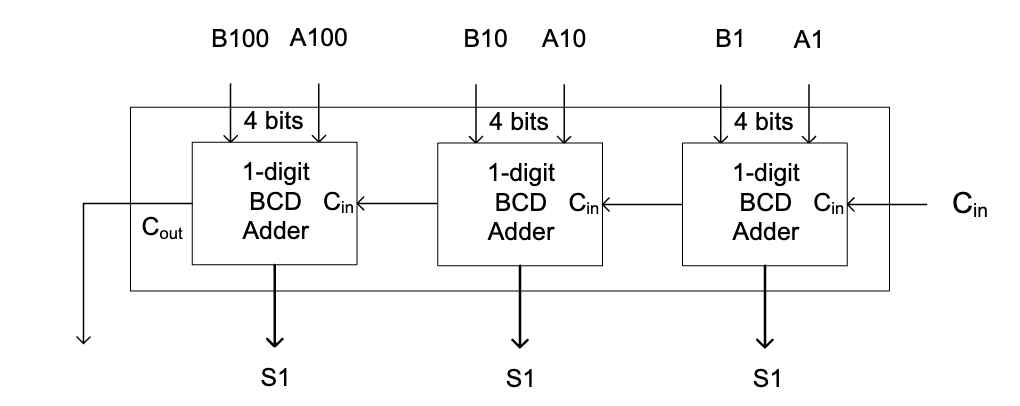
\includegraphics[width=0.8\textwidth]{figs/diagram.png}
\end{figure}


\subsubsection*{هدف آزمایش}

هدف از این آزمایش، آشنایی عملی با طراحی مدارهای منطقی ترکیبی سلسله‌مراتبی و پیاده‌سازی یک جمع‌کننده‌ی اعداد دهدهی کدشده به‌صورت \lr{BCD} (\lr{Binary Coded Decimal}) است. برخلاف جمع باینری معمولی، جمع دو رقم \lr{BCD} به یک مرحله‌ی تصحیح اضافه نیاز دارد تا نتیجه در بازه‌ی مجاز {(۰ تا ۹)} باقی بماند. اهداف مشخص این آزمایش عبارت‌اند از:

\begin{itemize}
  \item پیاده‌سازی یک تمام‌جمع‌کننده‌ی ۱ بیتی (\lr{Full Adder}) با گیت‌های پایه.
  \item طراحی مدار تصحیح \lr{BCD} برای جمع دو رقم دهدهی به‌همراه رقم نقلی ورودی.
  \item ساخت یک جمع‌کننده‌ی سه‌رقمی با زنجیر کردن سه نمونه از جمع‌کننده‌ی یک‌رقمی.
\end{itemize}


\subsubsection*{کدگذاری \lr{BCD}}

در کدگذاری \lr{BCD}، هر رقم دهدهی (۰ تا ۹) با ۴ بیت باینری نمایش داده می‌شود. برخلاف نمایش باینری خالص، در \lr{BCD} کدهای ۱۰۱۰ تا ۱۱۱۱ (معادل ۱۰ تا ۱۵) بلااستفاده و نامعتبر هستند.  هر رقم باید همیشه بین $0000_2$ تا $1001_2$ باشد.


\subsubsection*{جمع دو رقم \lr{BCD}}

اگر دو رقم \lr{BCD} (هرکدام حداکثر ۹) به‌همراه یک رقم نقلی ورودی (حداکثر ۱) با یک جمع‌کننده‌ی باینری معمولی ۴ بیتی جمع زده شوند، نتیجه‌ی خام می‌تواند تا:
\[
9 + 9 + 1 = 19
\]
برسد که در بازه‌ی معتبر \lr{BCD} (۰ تا ۹) نیست. اگر جمع خام از ۹ بیشتر باشد، باید مقدار ۶ ($0110_2$) به آن اضافه شود تا:
\begin{enumerate}
  \item رقم باقی‌مانده در بازه‌ی صحیح \lr{BCD} قرار بگیرد.
  \item یک رقم نقلی دهدهی (نه باینری) به رقم بعدی منتقل شود.
\end{enumerate}



\subsubsection*{تمام‌جمع‌کننده‌ی ۱ بیتی}

\begin{center}
\begin{tabular}{@{}lll@{}}
\toprule
\textbf{پایه} & \textbf{جهت} & \textbf{پهنا} \\
\midrule
\lr{A}, \lr{B}, \lr{Cin} & ورودی & ۱ بیت \\
\lr{Sum}, \lr{Cout} & خروجی & ۱ بیت \\
\bottomrule
\end{tabular}
\end{center}

مدار با ۲ گیت \lr{XOR}، ۲ گیت \lr{AND} و ۱ گیت \lr{OR} ساخته شده است:

\begin{itemize}
    \item $X_1 = A \oplus B$ \\
    نیمه‌جمع، بدون در نظر گرفتن رقم نقلی ورودی.

    \item $P_1 = A \land B$ \\
    آیا از جمع $A$ و $B$ به‌تنهایی رقم نقلی تولید می‌شود؟

    \item $\mathrm{Sum} = X_1 \oplus C_{in}$ \\
    جمع نهایی سه ورودی.

    \item $P_2 = X_1 \land C_{in}$ \\
    آیا از جمع $X_1$ و $C_{in}$ رقم نقلی تولید می‌شود؟

    \item $\mathrm{Cout} = P_1 \lor P_2$ \\
    رقم نقلی خروجی نهایی.
\end{itemize}

\begin{LTR}
\begin{center}
\begin{tabular}{@{}ccc|cc@{}}
\toprule
A & B & Cin & Sum & Cout \\
\midrule
0 & 0 & 0 & 0 & 0\\
0 & 0 & 1 & 1 & 0\\
0 & 1 & 0 & 1 & 0\\
0 & 1 & 1 & 0 & 1\\
1 & 0 & 0 & 1 & 0\\
1 & 0 & 1 & 0 & 1\\
1 & 1 & 0 & 0 & 1\\
1 & 1 & 1 & 1 & 1\\
\bottomrule
\end{tabular}
\end{center}
\end{LTR}

{
\centering{
  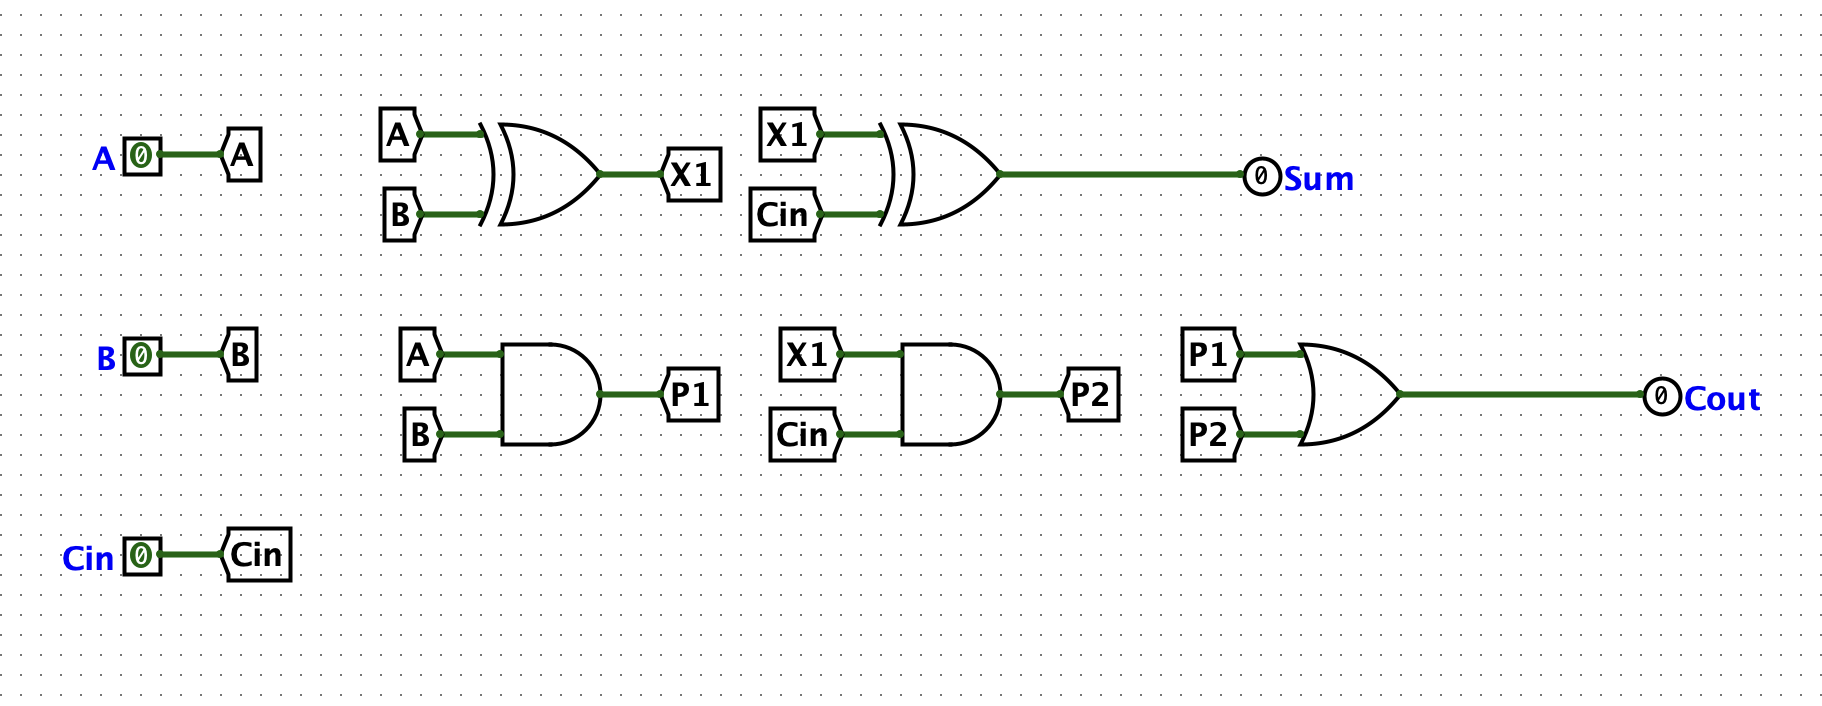
\includegraphics[width=0.8\textwidth]{figs/full-adder.png}
}
}



\subsubsection*{جمع‌کننده‌ی یک‌رقمی دهدهی}

\begin{center}
\begin{tabular}{@{}lll@{}}
\toprule
\textbf{پایه} & \textbf{جهت} & \textbf{پهنا} \\
\midrule
\lr{A}, \lr{B} & ورودی & ۴ بیت (رقم \lr{BCD}، ۰ تا ۹) \\
\lr{Cin} & ورودی & ۱ بیت \\
\lr{S} & خروجی & ۴ بیت (رقم نتیجه، ۰ تا ۹) \\
\lr{Cout} & خروجی & ۱ بیت (رقم نقلی دهدهی) \\
\bottomrule
\end{tabular}
\end{center}

این مدار در سه مرحله کار می‌کند که در ادامه هرکدام به‌طور کامل توضیح داده می‌شوند.

{مرحله‌ی اول: جمع باینری خام.}
ورودی‌های \lr{A} و \lr{B} با یک تفکیک‌کننده به بیت‌های تکی $A_0..A_3$ و $B_0..B_3$ شکسته می‌شوند و در زنجیره‌ی اول از ۴ تمام‌جمع‌کننده (\lr{FA0} تا \lr{FA3}) به‌صورت \lr{ripple-carry} جمع زده می‌شوند:

\begin{center}
\begin{tabular}{@{}lllll@{}}
\toprule
\textbf{نمونه} & \textbf{بیت} & \textbf{ورودی‌ها} & \textbf{خروجی جمع} & \textbf{رقم نقلی} \\
\midrule
\lr{FA0} & ۰ (کم‌ارزش) & $A_0, B_0, C_{in}$ & $S_0$ & $CY_0$ \\
\lr{FA1} & ۱ & $A_1, B_1, CY_0$ & $S_1$ & $CY_1$ \\
\lr{FA2} & ۲ & $A_2, B_2, CY_1$ & $S_2$ & $CY_2$ \\
\lr{FA3} & ۳ (پرارزش) & $A_3, B_3, CY_2$ & $S_3$ & $C_{outH}$ \\
\bottomrule
\end{tabular}
\end{center}

نتیجه‌ی این مرحله عدد ۴ بیتی $S_3 S_2 S_1 S_0$ (جمع باینری خام، {هنوز تصحیح‌نشده}) به‌همراه $C_{outH}$ (رقم نقلی خروجی این جمع ۴ بیتی، معادل وزن ۱۶) است.

{مرحله‌ی دوم: تشخیص نیاز به تصحیح.}
باید بررسی شود که آیا عدد $S_3S_2S_1S_0$ (با احتساب $C_{outH}$) از ۹ بزرگ‌تر است یا نه. چون $C_{outH}$ به‌تنهایی فقط سرریز $\geq 16$ را نشان می‌دهد، فرمول کمینه‌ی زیر برای پوشش کامل بازه‌ی ۱۰ تا ۱۹ استفاده شده است:

\[
CORR = C_{outH} \lor (S_3 \land S_2) \lor (S_3 \land S_1)
\] 

این فرمول با تنها ۳ گیت پیاده‌سازی شده است:

\begin{center}
\begin{tabular}{@{}llll@{}}
\toprule
\textbf{سیگنال} & \textbf{گیت} & \textbf{فرمول} & \textbf{معنی} \\
\midrule
\lr{G1OUT} & \lr{OR} & $S_2 \lor S_1$ & آیا یکی از بیت‌های ۱ یا ۲ روشن است؟ \\
\lr{G2OUT} & \lr{AND} & $S_3 \land {G1OUT}$ & آیا بیت ۳ \emph{و} یکی از بیت‌های ۱/۲ هم‌زمان روشن‌اند؟ \\
\lr{CORR} & \lr{OR} & $C_{outH} \lor {G2OUT}$ & سیگنال نهایی تصحیح \\
\bottomrule
\end{tabular}
\end{center}

سیگنال \lr{CORR} مستقیما به پایه‌ی خروجی \lr{Cout} این مدار وصل است؛ یعنی {رقم نقلی دهدهی، همان سیگنال تصحیح است.}

\textbf{چرا این فرمول درست کار می‌کند؟}

اگر $C_{outH}=1$، جمع خام حتما $\geq 16 > 9$ است. اگر $C_{outH}=0$، جمع خام حداکثر ۱۵ است؛ در این حالت باید $S_3=1$ باشد تا مقدار $\geq 8$ شود. با $S_3=1$: اگر $S_2=1$ مقدار حداقل ۱۲ است (همیشه $>9$)؛ اگر $S_2=0$ ولی $S_1=1$ مقدار حداقل ۱۰ است (باز هم $>9$). این دقیقا همان چیزی است که عبارت $(S_3\land S_2)\lor(S_3\land S_1)$ تشخیص می‌دهد.

{مرحله‌ی سوم: جمع تصحیحی $+6$.}
اگر $CORR=1$ باشد، باید مقدار ۶ (باینری $0110$) به عدد خام اضافه شود. چون بیت‌های ۰ و ۳ عدد ۶ صفر هستند، کافی است \lr{CORR} فقط به بیت‌های ۱ و ۲ اضافه شود  -  بدون نیاز به جمع‌کننده یا گیت \lr{AND} ۴ بیتی جداگانه. این کار با زنجیره‌ی دوم از ۴ تمام‌جمع‌کننده (\lr{FAC0} تا \lr{FAC3}) انجام می‌شود:

\begin{center}
\begin{tabular}{@{}lllllll@{}}
\toprule
\textbf{نمونه} & \textbf{بیت} & \textbf{ورودی} \lr{A} & \textbf{ورودی} \lr{B} & \lr{Cin} & \textbf{جمع نهایی} & \textbf{رقم نقلی} \\
\midrule
\lr{FAC0} & ۰ & $S_0$ & 0 & 0 & $SD_0$ & $CYC_0$ \\
\lr{FAC1} & ۱ & $S_1$ & \lr{CORR} & $CYC_0$ & $SD_1$ & $CYC_1$ \\
\lr{FAC2} & ۲ & $S_2$ & \lr{CORR} & $CYC_1$ & $SD_2$ & $CYC_2$ \\
\lr{FAC3} & ۳ & $S_3$ & 0 & $CYC_2$ & $SD_3$ & (استفاده نمی‌شود) \\
\bottomrule
\end{tabular}
\end{center}

بیت‌های $SD_0..SD_3$ (رقم نهایی و تصحیح‌شده) با یک تفکیک‌کننده‌ی ترکیبی به پایه‌ی خروجی \lr{S} وصل می‌شوند و هم‌زمان برای نمایش بصری به یک نمایشگر هفت‌قطعه‌ای (\lr{Hex Digit Display}) می‌روند.

\textbf{چرا رقم نقلی \lr{FAC3} استفاده نمی‌شود؟}

چون حداکثر مقدار ممکن در این جمع، $9+6=15$ است که همیشه در ۴ بیت جا می‌شود؛ بنابراین این جمع هرگز سرریز نمی‌کند.


{
	\centering{
  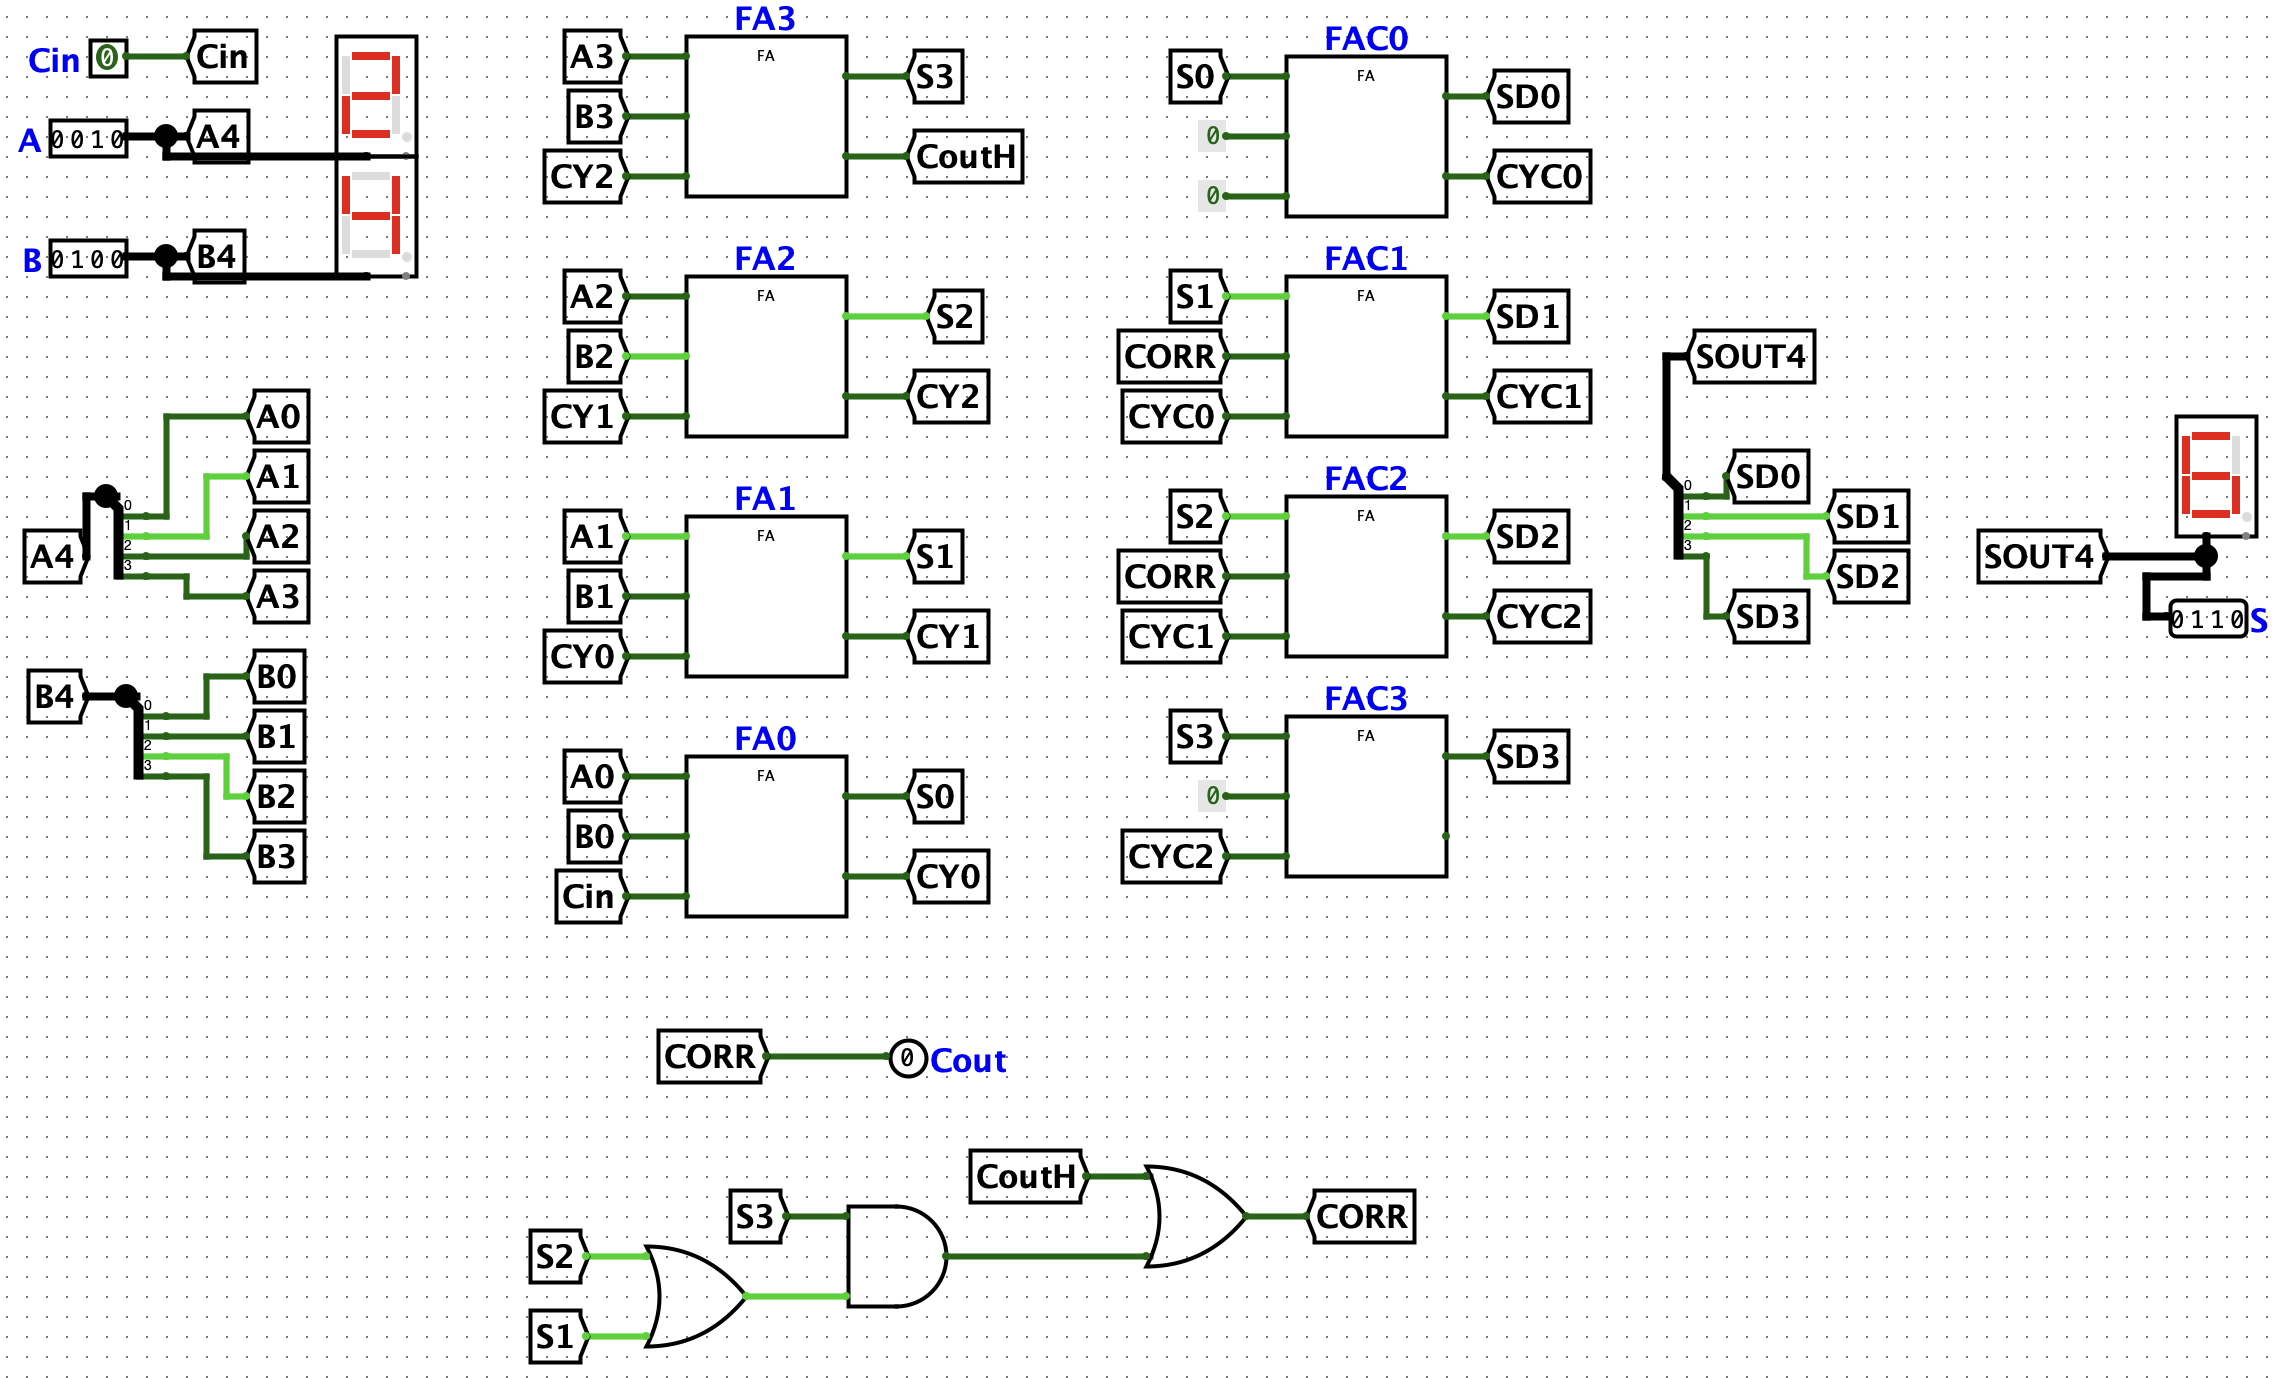
\includegraphics[width=1\textwidth]{figs/bcd-digit.png}
}
}


\pagebreak


\subsubsection*{مدار اصلی}

\begin{center}
\begin{tabular}{@{}lll@{}}
\toprule
\textbf{پایه} & \textbf{جهت} & \textbf{پهنا} \\
\midrule
\lr{A100}, \lr{A10}, \lr{A1} & ورودی & ۴ بیت هرکدام (رقم صدگان، دهگان، یکان عدد اول) \\
\lr{B100}, \lr{B10}, \lr{B1} & ورودی & ۴ بیت هرکدام (رقم صدگان، دهگان، یکان عدد دوم) \\
\lr{Cin} & ورودی & ۱ بیت \\
\lr{S100}, \lr{S10}, \lr{S1} & خروجی & ۴ بیت هرکدام \\
\lr{Cout} & خروجی & ۱ بیت \\
\bottomrule
\end{tabular}
\end{center}

سه نمونه از جمع‌کننده‌ی یک‌رقمی دهدهی دقیقا مانند جمع دستی چند رقمی روی کاغذ، به‌صورت زنجیره‌ای به هم وصل شده‌اند:

\begin{center}
\begin{tabular}{@{}llllll@{}}
\toprule
\textbf{نمونه} & \textbf{رقم} & \lr{A} & \lr{B} & \lr{Cin} & \lr{Cout} می‌رود به \\
\midrule
\lr{digit\_1} & یکان & \lr{A1} & \lr{B1} & \lr{Cin} (ورودی مدار) & تونل \lr{Cout1} \\
\lr{digit\_10} & دهگان & \lr{A10} & \lr{B10} & تونل \lr{Cout1} & تونل \lr{Cout10} \\
\lr{digit\_100} & صدگان & \lr{A100} & \lr{B100} & تونل \lr{Cout10} & پایه‌ی \lr{Cout} مدار \\
\bottomrule
\end{tabular}
\end{center}

هر رقم روی یک نمایشگر \lr{Hex Digit Display} جداگانه نشان داده می‌شود و \lr{Cout} نهایی به یک \lr{LED} وصل است (در صورت سرریز از عدد ۹۹۹، روشن می‌شود).


{
	\centering{
  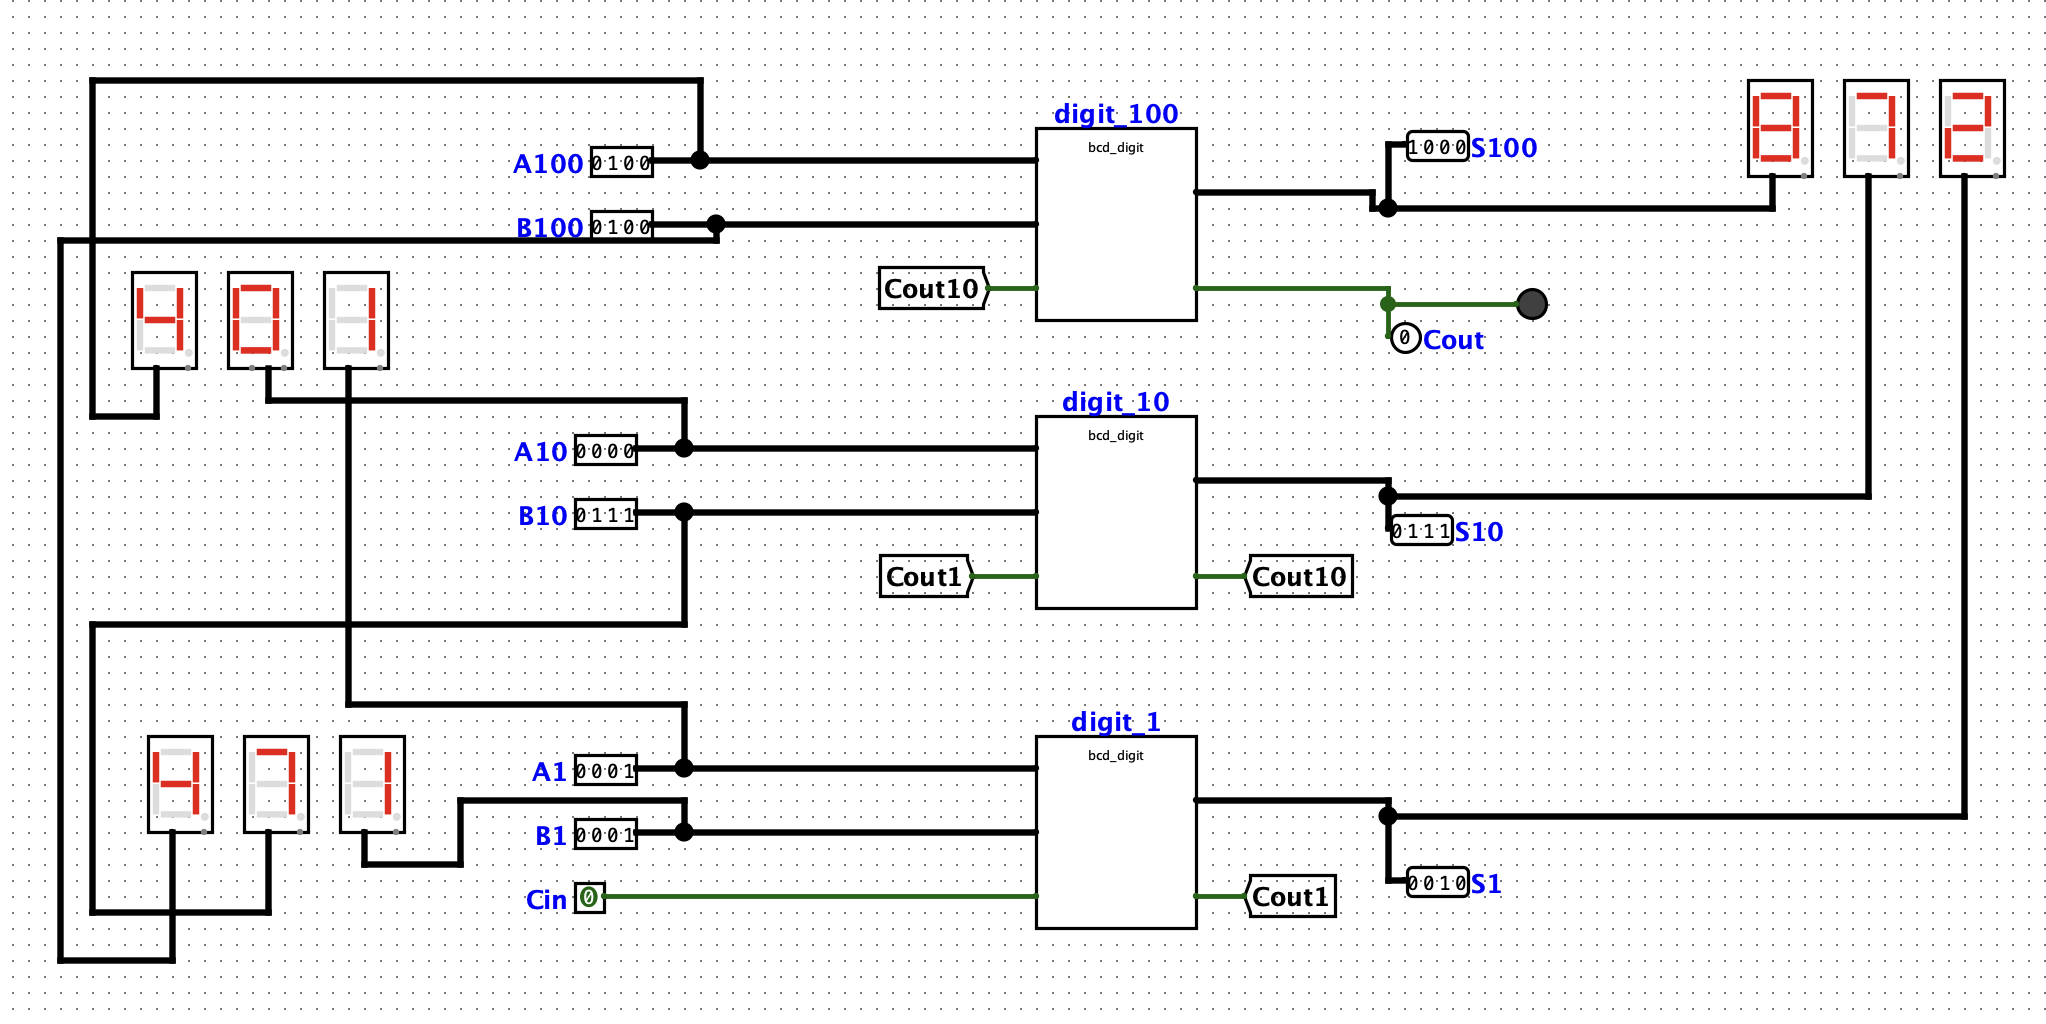
\includegraphics[width=1\textwidth]{figs/main.png}
}
}

\subsubsection*{ نتایج تست}

هر سه مدار با بردار تست و از طریق خط فرمان \lr{Logisim} در حالت \lr{headless} تست شدند. 


\end{document}